\section{Auswertung}
\subsection{Dioden}
\begin{enumerate}[label=\alph*)]
	\item Stellen Sie die Kennlinien im linearen Maßstab dar, benutzen Sie dazu die korrigierten Messwerte (Spannungsfehlerschaltung beachten, Durchlassrichtung und Sperrrichtung unterschiedliche Maßstäbe, ggf. je zwei Diagramme).
% \newcommand\myeq{\stackrel{{{m}}}{=}}
    % \begin{align*}
    %   x &\myeq 10
    % \end{align*}
	      \begin{figure}[h!]
		      \begin{center}
			      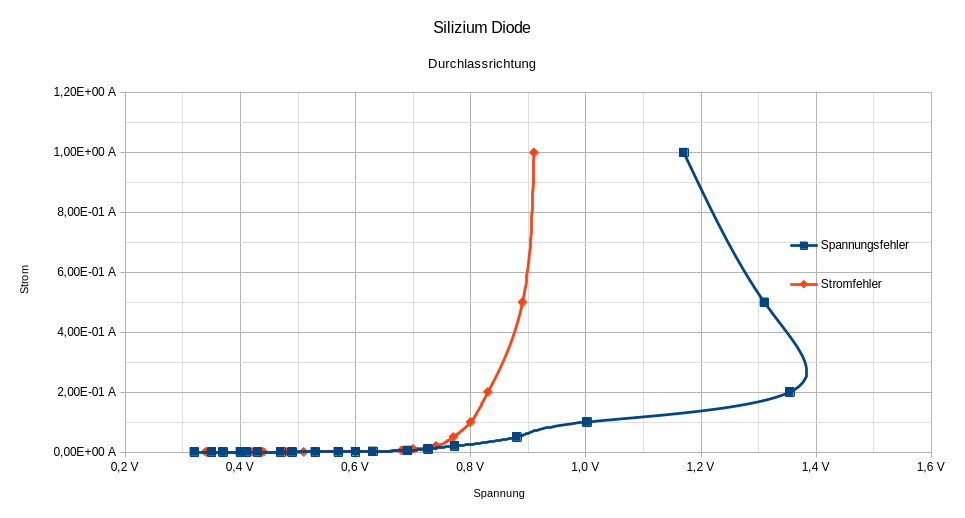
\includegraphics[width=0.85\textwidth]{img/4.1.a.1}
			      \caption{Silizium Diode in Durchlassrichtung}
		      \end{center}
	      \end{figure}

	      \begin{figure}[h!]
		      \begin{center}
			      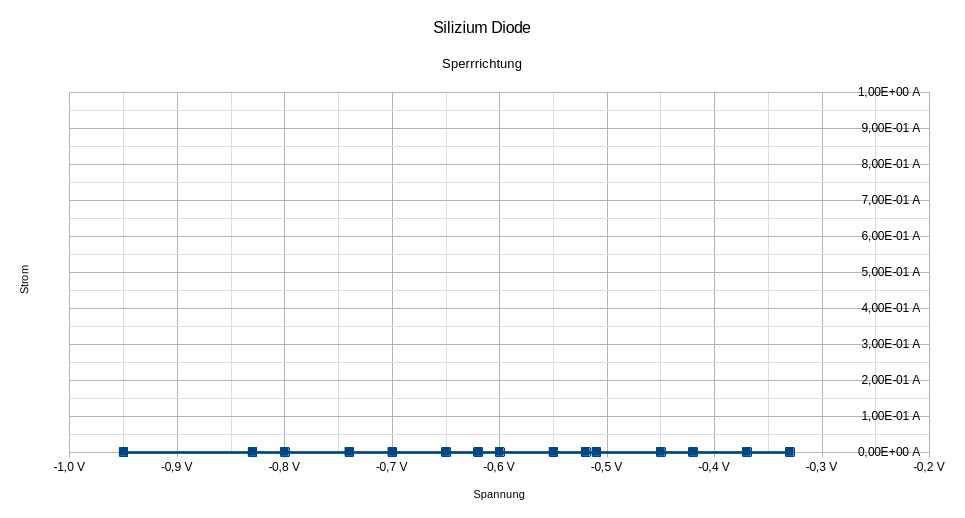
\includegraphics[width=0.85\textwidth]{img/4.1.a.2}
			      \caption{Silizium Diode in Sperrrichtung}
		      \end{center}
	      \end{figure}

	      \pagebreak

	      \begin{figure}[h!]
		      \begin{center}
			      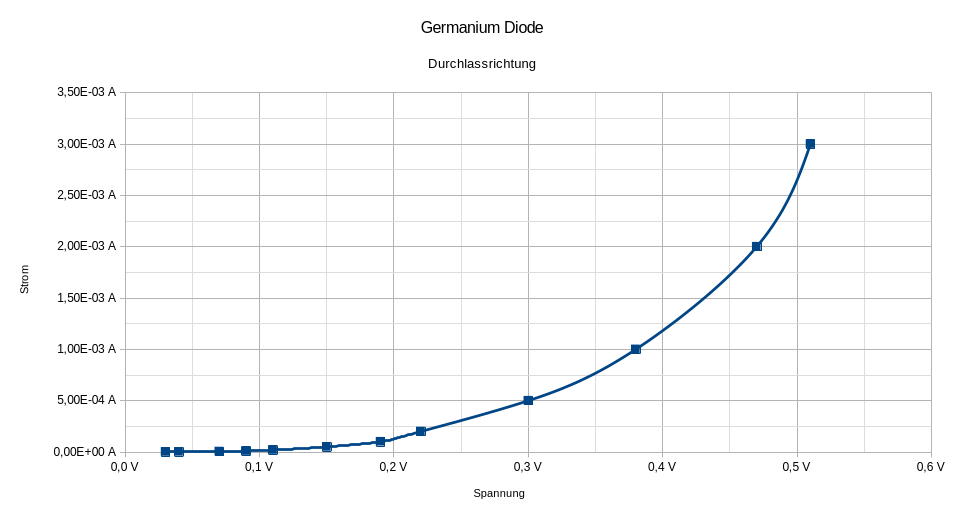
\includegraphics[width=0.85\textwidth]{img/4.1.a.3}
			      \caption{Germanium Diode in Durchlassrichtung}
		      \end{center}
	      \end{figure}

	      \begin{figure}[h!]
		      \begin{center}
			      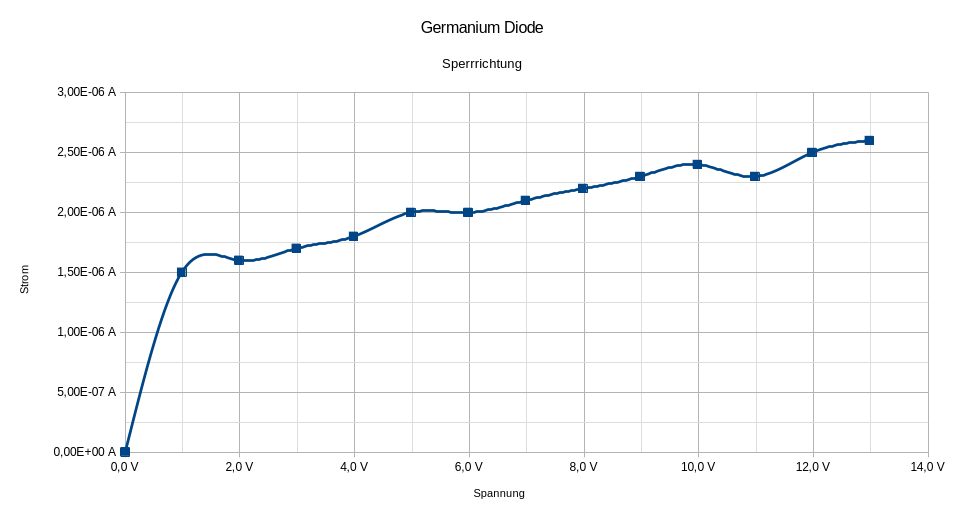
\includegraphics[width=0.85\textwidth]{img/4.1.a.4}
			      \caption{Germanium Diode in Sperrrichtung}
		      \end{center}
	      \end{figure}

	      \pagebreak

	      \begin{figure}[h!]
		      \begin{center}
			      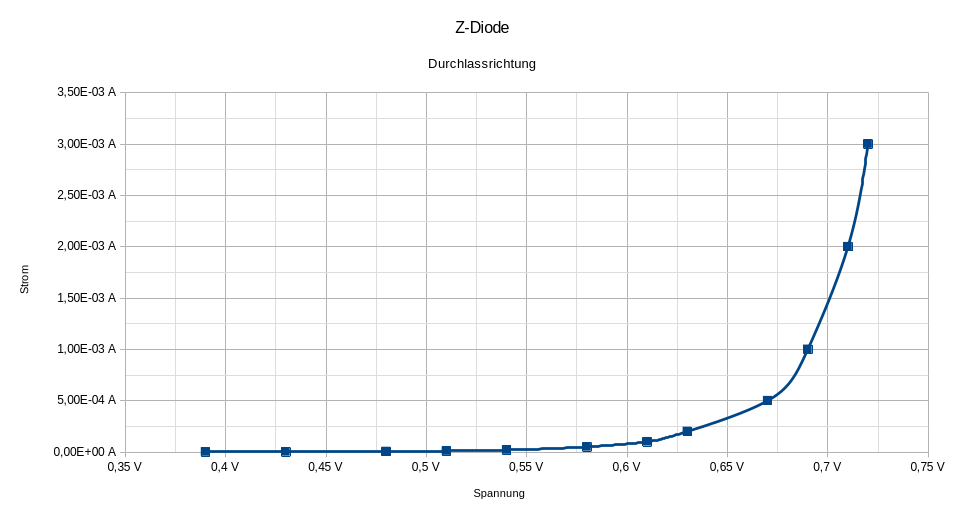
\includegraphics[width=0.85\textwidth]{img/4.1.a.5}
			      \caption{Z-Diode in Durchlassrichtung}
		      \end{center}
	      \end{figure}

	      \begin{figure}[h!]
		      \begin{center}
			      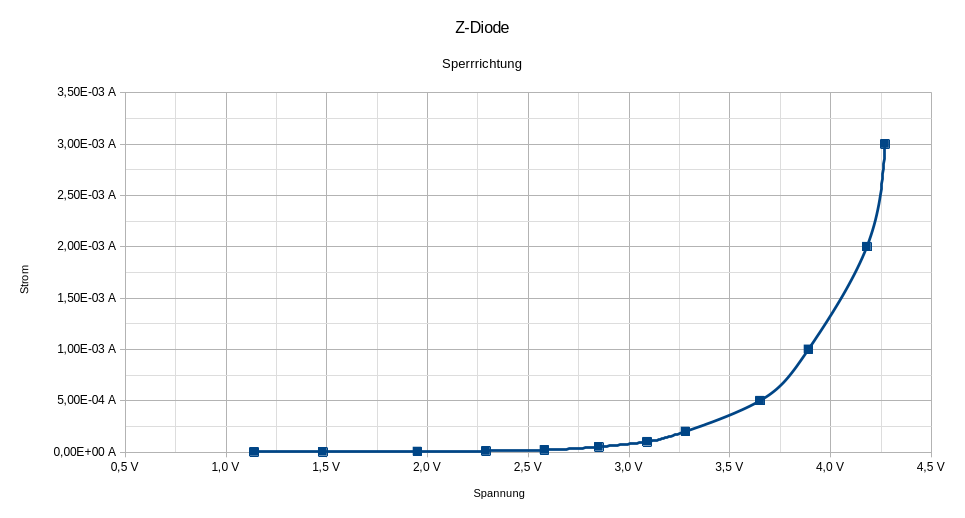
\includegraphics[width=0.85\textwidth]{img/4.1.a.6}
			      \caption{Z-Diode in Sperrrichtung}
		      \end{center}
	      \end{figure}

	      \pagebreak
	\item Berechnen Sie die Kennlinie der Si-Diode nach Gleichung 7, ermitteln Sie den Sperrstrom $I_s$ und den Emissionskoeffizienten m aus den Messungen. (Tipp: Den Emissionskoeffizienten bestimmen Sie, indem Sie zwei Messwerte in Gleichung 7 einsetzen und beide Gleichungen dividieren, so dass der Sperrstrom gekürzt werden kann. Diese Gleichung kann nun nach $m$ umgestellt werden.)
	      \begin{align*}
		      % I_1             & =I_s \cdot \left(e^\frac{U_1}{m\cdot U_T} - 1 \right)         \\
		      % I_2             & =I_s \cdot \left(e^\frac{U_2}{m\cdot U_T} - 1 \right)         \\
		      \frac{I_1}{I_2} & = \frac{I_s \cdot \left(e^\frac{U_1}{m\cdot U_T} - 1 \right)}
		      {I_s \cdot \left(e^\frac{U_2}{m\cdot U_T} - 1 \right)}                          \\
		      \frac{I_1}{I_2} & = \frac{e^\frac{U_1}{m\cdot U_T} - 1 }
		      {e^\frac{U_2}{m\cdot U_T} - 1}                                                  \\
	      \end{align*}
	      Die Rechnung lässt sich viel vereinfachen, wenn $\displaystyle{e^\frac{U}{m\cdot U_t} >> 1}$ ist. \\
	      Annahme: $m = m_{max} = 2$ und $10^3 >> 1$
	      \begin{align*}
		      e^\frac{U_{min}}{m_{max}\cdot U_t}         & \geq 10^3                                                    \\
		      \frac{U_{min}}{m_{max}\cdot U_t}           & \geq 3\cdot \ln(10)                                          \\
		      \frac{U_{min}}{2\cdot 25,3\cdot10^{-3}\ V} & \geq 3\cdot \ln(10)                                          \\
		      U_{min}                                    & \geq \frac{151,8\cdot \ln(10)}{10^3}\ V                      \\
		      U_{min}                                    & \geq 0,35\ V                                                 \\
		      \Rightarrow
		      \frac{I_1}{I_2}                            & = \frac{e^\frac{U_1}{m\cdot U_T}}
		      {e^\frac{U_2}{m\cdot U_T}}                                                                                \\
		      \frac{I_1}{I_2}                            & = e^\frac{U_1-U_2}{m\cdot U_T}                               \\
		      \ln\left(\frac{I_1}{I_2}\right)            & =  \frac{U_1-U_2}{m\cdot U_T}                                \\
		      m                                          & =  \frac{U_1-U_2}{\ln\left(\frac{I_1}{I_2}\right) \cdot U_T} \\
		      m                                          & =  \frac{0,4\ V - 0,89\ V}
		      {\ln\left(\frac{5\ \mu A}{0,5\ A}\right) \cdot 25\cdot 10^{-3}\ V} = 1,68                                 \\
		      I_s                                        & = \frac{I_1}{e^\frac{U_1}{m\cdot U_T} - 1}                   \\
		      I_s                                        & = \frac{5\ \mu A}{e^\frac{0,4\ V}
		      {1,68\cdot 25,3\cdot 10^{-3}\ V} - 1} = 4,029\cdot 10^{-10} A                                             \\
		      % I                                          & = 4,029\cdot 10^{-10}\ A\cdot
		      % \left(e^{\frac{U}{1,68\cdot 25,3\cdot 10^{-3}\ V}}-1\right)                                               \\
		      I                                          & = 4,029\cdot 10^{-10}\ A\cdot
		      \left(e^{\frac{U}{42,5\cdot 10^{-3}\ V}}-1\right)
	      \end{align*}
  \pagebreak

	\item Stellen Sie die gemessene und berechnete Kennlinie der Si-Diode im halblogarithmischen Maßstab dar (berechnete Kennlinie als Linie, Messwerte als Punkte).

	      \begin{figure}[h!]
		      \begin{center}
			      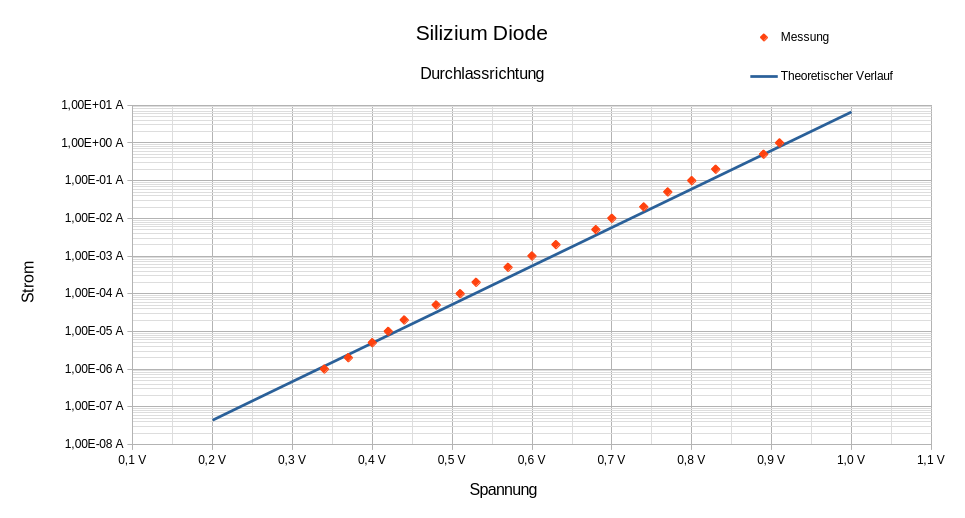
\includegraphics[width=0.85\textwidth]{img/4.1.a.7}
			      \caption{Kennlinie der Si-Diode aus dem theoretischem Verlauf und der Messungen}
		      \end{center}
	      \end{figure}

	\item Beschriften Sie die fünf aufgenommenen Oszillogramme eindeutig.

	      \begin{figure}[h!]
		      \begin{center}
            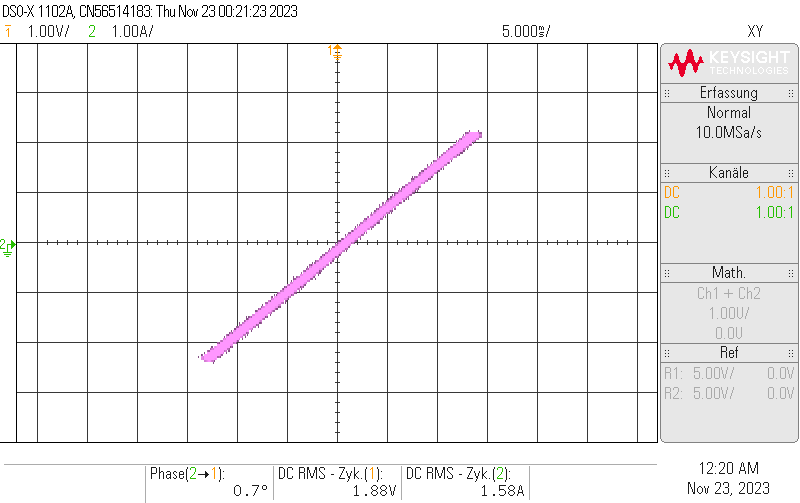
\includegraphics[width=0.85\textwidth]{img/V1/3.2.Widerstand.png}
			      \caption{Oszillogramm des ohmschen Widerstands}
		      \end{center}
	      \end{figure}

\pagebreak
	      \begin{figure}[h!]
		      \begin{center}
			      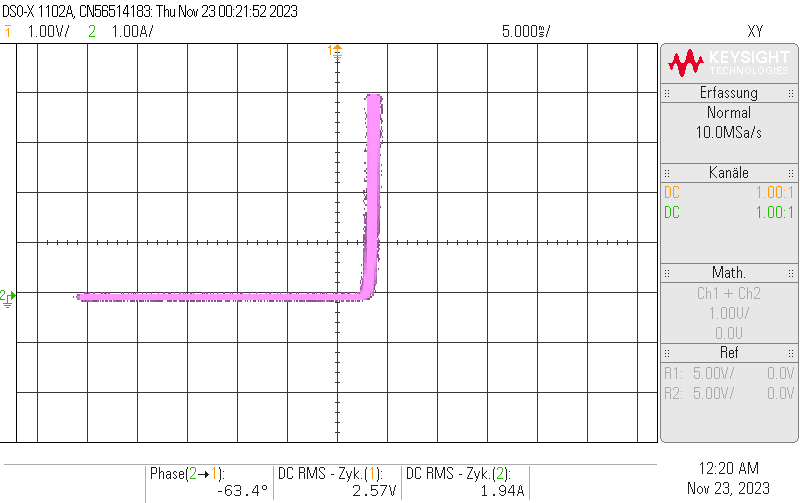
\includegraphics[width=0.85\textwidth]{img/V1/3.2.Diode_Si.png}
			      \caption{Oszillogramm der Si-Diode}
		      \end{center}
	      \end{figure}

	      \begin{figure}[h!]
		      \begin{center}
			      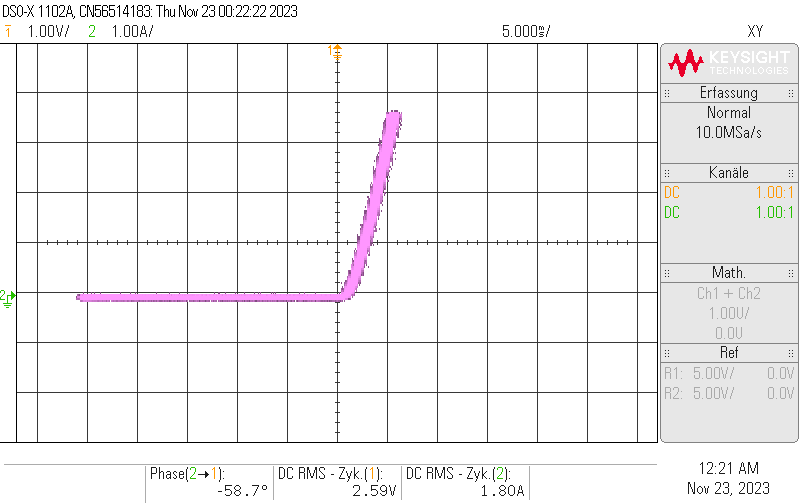
\includegraphics[width=0.85\textwidth]{img/V1/3.2.Diode_Ge.png}
			      \caption{Oszillogramm der Germanium-Diode}
		      \end{center}
	      \end{figure}

\pagebreak
	      \begin{figure}[h!]
		      \begin{center}
			      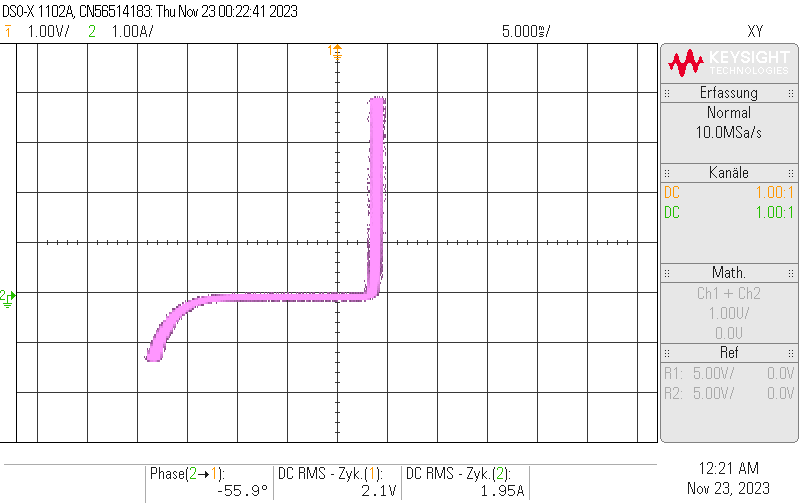
\includegraphics[width=0.85\textwidth]{img/V1/3.2.Diode_Ze.png}
			      \caption{Oszillogramm der Z-Diode}
		      \end{center}
	      \end{figure}

	      \begin{figure}[h!]
		      \begin{center}
			      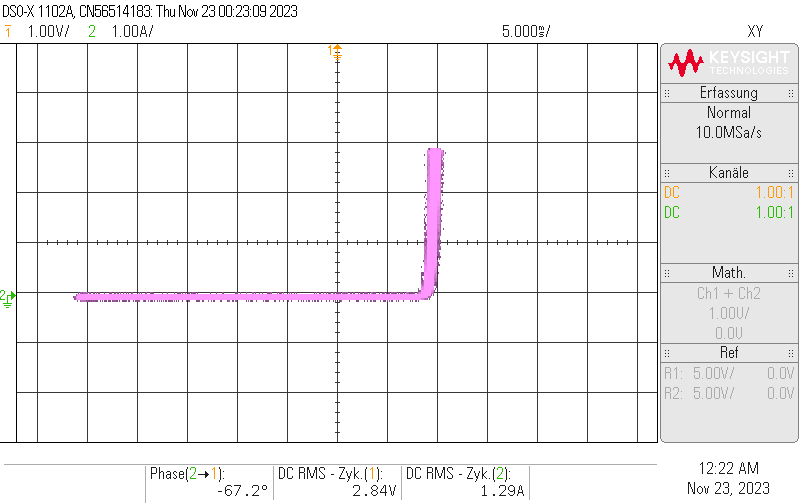
\includegraphics[width=0.85\textwidth]{img/V1/3.2.Diode_Led.png}
			      \caption{Oszillogramm der Leuchtdiode}
		      \end{center}
	      \end{figure}
\end{enumerate}

\pagebreak
\subsection{Temperaturabhängiger Widerstand}
\begin{enumerate}[label=\alph*)]
	\item Ermitteln Sie für jeden Messwert den Widerstand (Spannungsfehlerschaltung beachten!)
	      \begin{table}[h!]
		      \caption{Temperaturabhängiger Widerstand: Strom- und Widerstandswerte}
		      \begin{center}
			      \begin{tabular}[c]{c|c|c}
				      \hline
				      \multicolumn{1}{c|}{\textbf{Temperatur in $^\circ C$}} &
				      \multicolumn{1}{c|}{\textbf{Strom in $mA$}}            &
				      \multicolumn{1}{c}{\textbf{Widerstand in $\Omega$}}                     \\
				      \hline
				      22,5                                                   & 2    & 1000,00 \\
				      25                                                     & 2,2  & 909,09  \\
				      30                                                     & 2,4  & 833,33  \\
				      35                                                     & 2,7  & 740,74  \\
				      40                                                     & 2,9  & 689,66  \\
				      45                                                     & 3,5  & 571,43  \\
				      50                                                     & 4    & 500,00  \\
				      55                                                     & 5    & 400,00  \\
				      60                                                     & 6    & 333,33  \\
				      65                                                     & 6,7  & 298,51  \\
				      70                                                     & 8,6  & 232,56  \\
				      75                                                     & 10   & 200,00  \\
				      80                                                     & 10,5 & 190,48  \\
				      85                                                     & 13   & 153,85  \\
				      90                                                     & 15   & 133,33  \\
				      95                                                     & 20   & 100,00  \\
				      100                                                    & 35   & 57,14   \\
				      \hline
			      \end{tabular}
		      \end{center}
	      \end{table}
	      \begin{figure}[h!]
		      \begin{center}
			      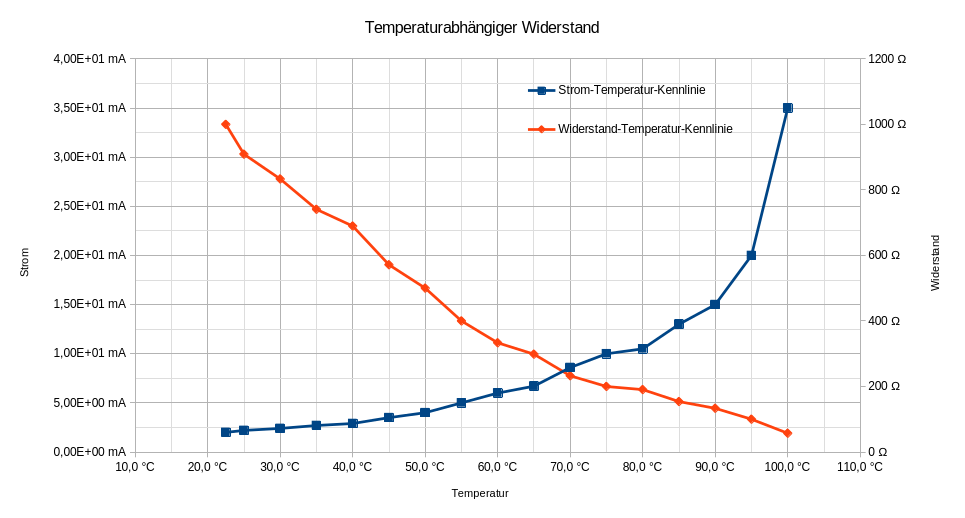
\includegraphics[width=0.95\textwidth]{img/4.2.a.1}
		      \end{center}
		      \caption{Strom-Temperatur-Kennlinie und Widerstand-Temperatur-Kennlinie}
	      \end{figure}
	      \pagebreak

	\item Berechnen Sie die Widerstandskennlinie näherungsweise nach Gleichung 8. Die Werkstoffkonstanten A und B sind aus den Messwerten bei minimaler und maximaler Temperatur zu ermitteln.
	      \begin{align*}
		      R(T)                                    & = A\cdot e^{\frac{B}{T}}                                                                \\
		      A                                       & = \frac{R(T)}{e^{\frac{B}{T}}}                                                          \\
		      \frac{R(T_1)}{R(T_2)}                   & = \frac{A}{A} \cdot \frac{e^{\frac{B}{T_1}}}{e^{\frac{B}{T_2}}}                         \\
		      \frac{R(T_1)}{R(T_2)}                   & = e^{\frac{B\cdot T_2-B\cdot T_1}{T_1\cdot T_2}}                                        \\
		      \ln \left(\frac{R(T_1)}{R(T_2)} \right) & = {\frac{B\cdot( T_2- T_1)}{T_1\cdot T_2}}                                              \\
		      B                                       & =\frac{\ln \left(\frac{R(T_1)}{R(T_2)} \right)\cdot {T_1\cdot T_2}}{( T_2- T_1)}        \\
		      B                                       & =\frac{\ln \left(\frac{1000\ \Omega}{57,14\ \Omega}\right)
		      \cdot {(295,65\ K \cdot 374,15\ K)}}{(374,15\ K - 295,65\ K)}                                                                     \\
		      B                                       & =4033\ K                                                                                \\
		      A                                       & = \frac{R(T_1)}{e^{\frac{B}{T_1}}} = \frac{1000\ \Omega}{e^{\frac{4033\ K}{295,65\ K}}} \\
		      A                                       & = 1,19\ m\Omega                                                                         \\
		      R(T)                                    & = 1,19\ m\Omega \cdot e^{\frac{4033\ K}{T}}                                             \\
	      \end{align*}
	\item Stellen Sie beide Kennlinien in einem Diagramm da (berechnete Kennlinie als Linie, Messwerte als Punkte).
	      \begin{figure}[h!]
		      \begin{center}
			      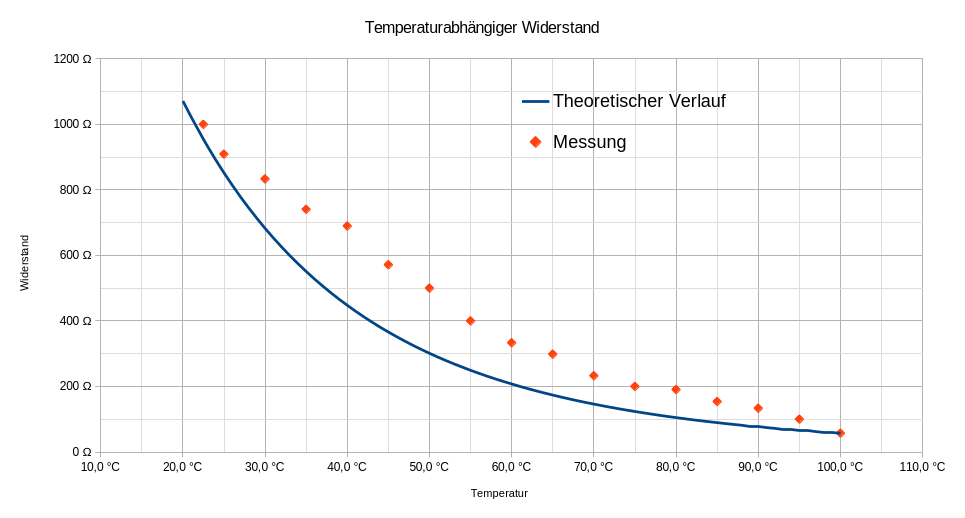
\includegraphics[width=0.7\textwidth]{img/4.2.c.1}
		      \end{center}
		      \caption{Widerstandskennlinie aus dem theoretischem Verlauf und der Messungen}\label{img:4.2.c.1}
	      \end{figure}

	      \pagebreak
	\item Vergleichen Sie die Kennlinien.
\end{enumerate}


\pagebreak
\subsection{Transistor}
\begin{enumerate}[label=\alph*)]
	\item Stellen Sie die Eingangskennlinien nach 3.4.1 im linearen Maßstab in einem Diagramm dar.
	      \begin{figure}[h!]
		      \begin{center}
			      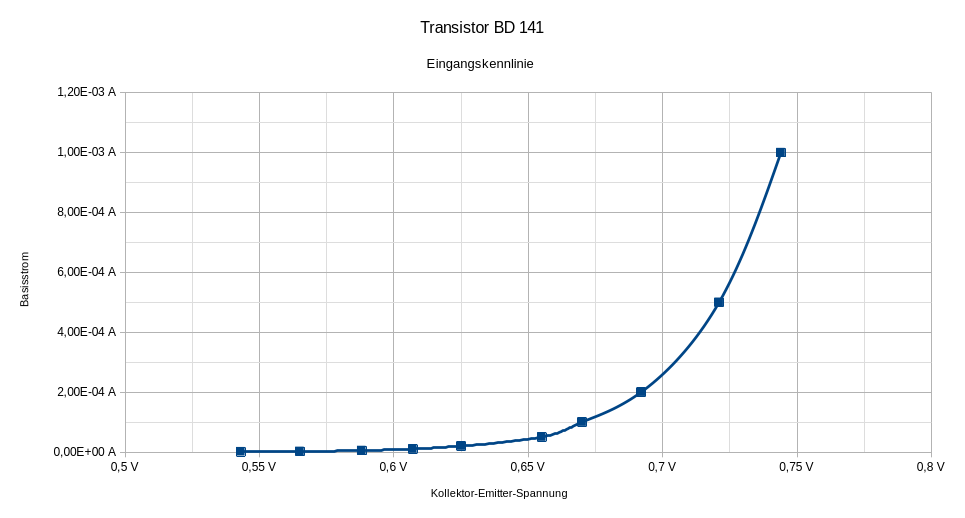
\includegraphics[width=0.85\textwidth]{img/4.3.a.1}
		      \end{center}
		      \caption{Eingangskennlinien des Transistors}
	      \end{figure}

	\item Stellen Sie das Ausgangskennlinienfeld nach 3.4.2 im linearen Maßstab in einem Diagramm dar.
	      \begin{figure}[h!]
		      \begin{center}
			      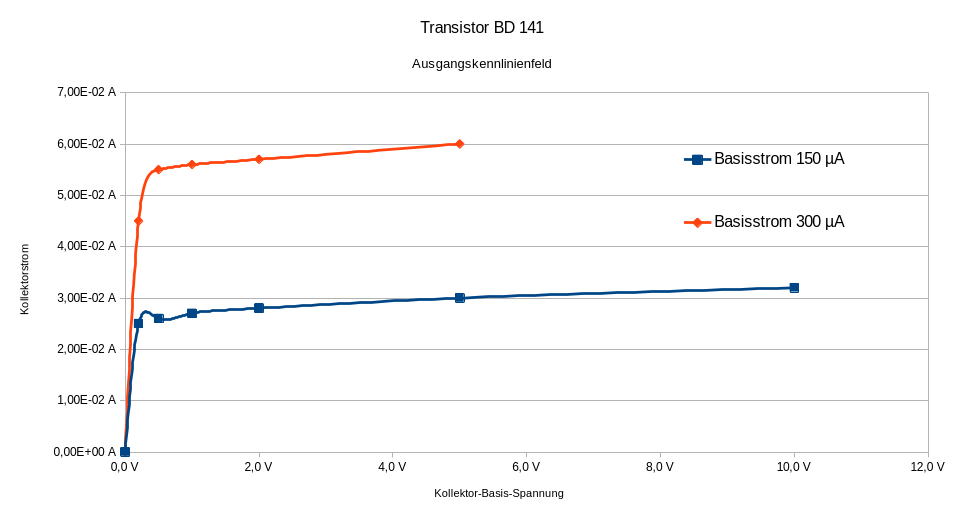
\includegraphics[width=0.85\textwidth]{img/4.3.b.1}
		      \end{center}
		      \caption{Ausgangskennlinienfeld des Transistors}
	      \end{figure}

  \pagebreak
	\item Beschriften Sie das aufgenommene Oszillogramm eindeutig.
	      \begin{figure}[h!]
		      \begin{center}
			      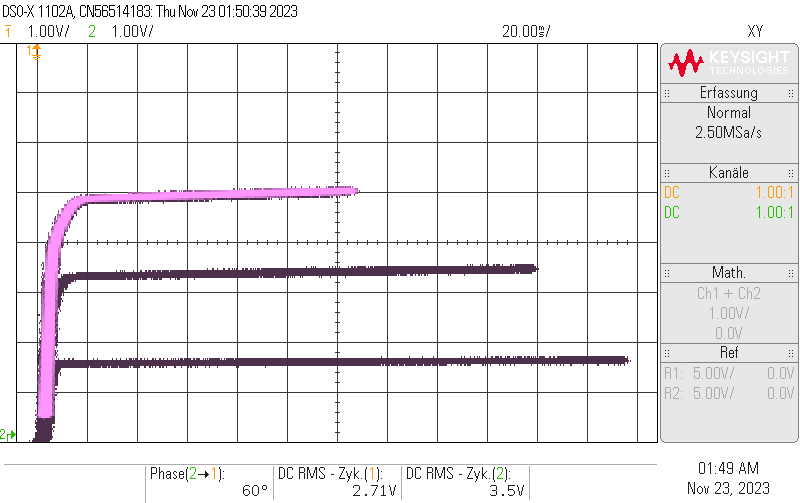
\includegraphics[width=0.85\textwidth]{img/V1/Ausgang.png}
		      \end{center}
		      \caption{Oszillogramm der Ausgangskennlinienfelder}
	      \end{figure}
\end{enumerate}
